\subsubsection{Begreper}
TODO

\subsubsection{Firkantbølge fra sinusbølger}
Ved å generere to sinusbølger
kan man addere dem sammen for å tilnærme en firkantbølge.
\\
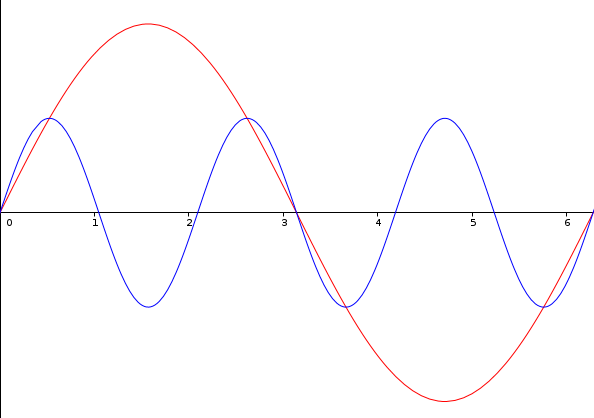
\includegraphics[width=\textwidth]{./img/harmoni-ab}
Vi har to funksjoner: \\
{\color{red} $a = 2\sin{x}$} \\
{\color{blue} $b = \sin{3x}$}
\\
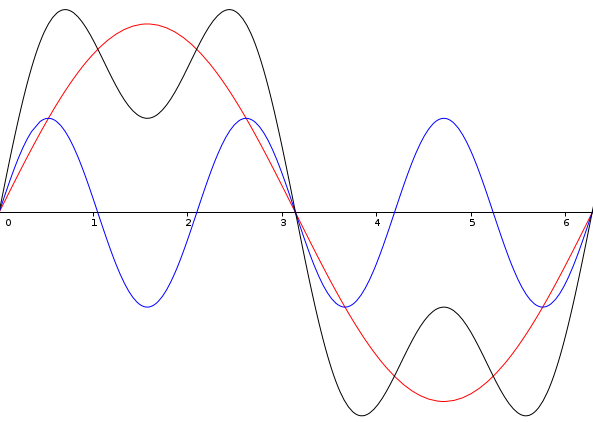
\includegraphics[width=\textwidth]{./img/harmoni-abc}
Lagt sammen blir \\
$c = $ {\color{red} $a$} $+$ {\color{blue} $b$} \\
Du kan se at det begynner å ligne på en firkantbølge.
